% file: graphs_v8_r3_rep_12_2.tex
% created by Orbiter tikz interface
% creation date: Sat Jul 30 08:32:03 +03 2022
% DeviceCoordinates 0 0 1000000 1000000
% UserCoordinates 0 0 10000 10000
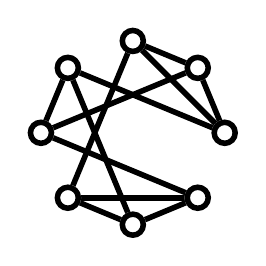
\begin{tikzpicture}[scale=0.1,line width = 2pt]
\draw [] (28.3333,16.6667) -- (24.9133,24.9133);
\draw [] (28.3333,16.6667) -- (16.6667,28.3333);
\draw [] (28.3333,16.6667) -- (8.42,24.9133);
\draw [] (24.9133,24.9133) -- (16.6667,28.3333);
\draw [] (24.9133,24.9133) -- (5,16.6667);
\draw [] (16.6667,28.3333) -- (8.42,8.42);
\draw [] (8.42,24.9133) -- (5,16.6667);
\draw [] (8.42,24.9133) -- (16.6667,5);
\draw [] (5,16.6667) -- (24.9133,8.42);
\draw [] (8.42,8.42) -- (16.6667,5);
\draw [] (8.42,8.42) -- (24.9133,8.42);
\draw [] (16.6667,5) -- (24.9133,8.42);
\filldraw[color=white] (28.3333,16.6667) circle [radius = 1.33333cm];
\draw (28.3333,16.6667) circle [radius = 1.33333cm];
\filldraw[color=white] (24.9133,24.9133) circle [radius = 1.33333cm];
\draw (24.9133,24.9133) circle [radius = 1.33333cm];
\filldraw[color=white] (16.6667,28.3333) circle [radius = 1.33333cm];
\draw (16.6667,28.3333) circle [radius = 1.33333cm];
\filldraw[color=white] (8.42,24.9133) circle [radius = 1.33333cm];
\draw (8.42,24.9133) circle [radius = 1.33333cm];
\filldraw[color=white] (5,16.6667) circle [radius = 1.33333cm];
\draw (5,16.6667) circle [radius = 1.33333cm];
\filldraw[color=white] (8.42,8.42) circle [radius = 1.33333cm];
\draw (8.42,8.42) circle [radius = 1.33333cm];
\filldraw[color=white] (16.6667,5) circle [radius = 1.33333cm];
\draw (16.6667,5) circle [radius = 1.33333cm];
\filldraw[color=white] (24.9133,8.42) circle [radius = 1.33333cm];
\draw (24.9133,8.42) circle [radius = 1.33333cm];
\end{tikzpicture}
